\documentclass[12pt]{article}
\usepackage[utf8]{inputenc}
\usepackage[russian]{babel}
\usepackage{multicol}
\usepackage[papersize={21cm, 36cm}, left=10mm, top=15mm, right=15mm, bottom=25mm]{geometry}
\usepackage{mathtools}
\documentclass[captions=tableheading]{scrbook}
\usepackage{caption}
\usepackage{tikz} 
\usepackage{amsmath}
\usepackage{graphicx}
\usepackage{wrapfig}
\graphicspath{{pictures/}}
\usepackage[usenames]{color}
\usepackage[most]{tcolorbox}
\usepackage{colortbl}
\usepackage{fancyhdr}
\usepackage{float}
\usepackage[leftcaption]{sidecap}
\setlength{\columnsep}{1cm}
\DeclareGraphicsExtensions{.png}
\usepackage{afterpage}
\fancypagestyle{mystile}{
\fancyhf{}
\fancyfoot[r]{\textbf{47}}
\renewcommand{\headrulewidth}{0pt}
\fancyhead{}
}
\pagestyle{mystile}

\begin{document}
\begin{multicols}{2}
\setcounter{figure}{5}
\begin{figure}[H]
    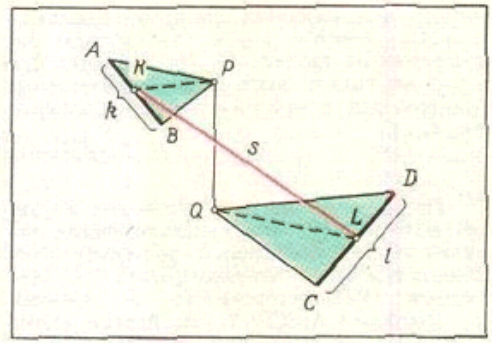
\includegraphics[scale=0.5]{ris6.png}
    \captionsetup{singlelinecheck=off}
    \caption{}
    \label{fig:ris6}
\end{figure}

\parindent0pt
лежать отрезки $a$ и $b$. (В этой и следующих)\linebreak
формулах $a$, пр $b$ и т.п. ознают длины со-\linebreak
ответствующих отрезков.) Наименьший угол\linebreak
между прямыми не превосходит $\pi$/2, поэто-\linebreak
му $\mathrm{cos\alpha \ge 0}$. Из (1) следует равенство \\
\setcounter{equation}{1}
\begin{equation}
    \label{eq:eq2}
    a \text{ пр}_{a}{b} = b \text{ пр}_{\alpha}a,
\end{equation}
которое пригодится нам при решении задачи.\linebreak
\rule{0.85cm} ООбозначим через $P$ центр верхнего, а\linebreak
через $Q^{\prime}$ — центр нижнего оснований пирами-\linebreak
ды. Мы докажем следующий факт, несколь-\linebreak
ко более общий, чем нужное нам утвержде-\linebreak
ние задачи \textbf{M168}. \\
\rule{0.85cm} ППусть плоскости двух подобных равно-\linebreak
бедренных треугольников $ABP$ и $CDQ$ с вер-\linebreak
шинами $P$ и $Q$ перпендикулярны отрезку $PQ$\linebreak
(и, тем самым, параллельны между собой).\linebreak
Обозначим отрезок, соединяющий середины\linebreak
$K$ и $L$ оснований $AB$ и $CD$ через $s$ Тогда\linebreak
(рис. \ref{fig:ris6}).
%\equation\text{ пр}_{s}{k} = \text{ пр}_{s}{l},\label{eq:test}\eqno(3)
\begin{equation}
    \label{eq:eq3}
    \text{ пр}_{s}{k} = \text{ пр}_{s}{l},
\end{equation}
Пользуясь \eqref{eq:eq2}, мы вместо \eqref{eq:eq3} можем доказы-\linebreak
вать такое равенство:
\begin{equation}
    \label{eq:eq4}
    k \text{ пр}_{k}{s} = t\text{ пр}_{t}{s},
\end{equation}
Теперь воспользуемся тем, что как это сле-\linebreak
дует из (1), длина пр $b_{a}$ не меняется при па-\linebreak
раллельном переносе отрезков $а$ и $b$. Поэто-\linebreak
му мы можем спроектировать отрезок $k=AB$\linebreak
на плоскость, треугольника $CDQ$ и получим:
\begin{multline}
\large{\text{ пр}_{A^{\prime}B^{\prime}}K^{\prime}L = \text{ пр}_{^{\prime}B^{\prime}}KL = \text{ пр}_{AB}KL = \\ 
= \text{ пр}_{k}{s},}
\label{eq:eq5}
\end{multline}
\begin{figure}[H]
    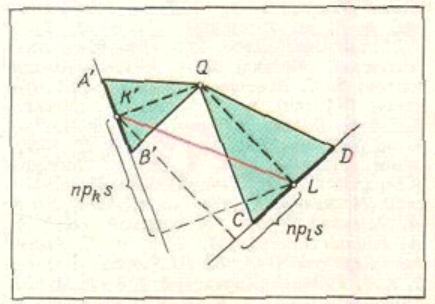
\includegraphics[scale=0.6]{ris7.png}
    \captionsetup{singlelinecheck=off}
    \caption{}
    \label{fig:ris7}
\end{figure} 

%\begin{left}
%\end{left}

\parindent0pt
где $A^{\prime}$, $B^{\prime}$ и $K^{\prime}$ $-$ проекции точек $A$, $B$ и $K$\linebreak
на плоскость $CDQ$ (рис. \ref{fig:ris7}). Таким образом,\linebreak
мы свели задачу к тому случаю, когда оба\linebreak
треугольника лежат в одной плоскости (и име-\linebreak
ют общую вершину).

\rule{0.85cm} ЕЕсли отрезки $AB$ и $CD$ параллельны,\linebreak
то равенство \eqref{eq:eq4} очевидно, поскольку обе\linebreak
проекции равны нулю. Если эти отрезки не-\linebreak
параллельны, то получаем:
\begin{multline}
\displaymath\large{\frac{k}{l}=\frac{A^{\prime}B^{\prime}}{CD}=\frac{QK^{\prime}}{QL}=\frac{\sin \angle QLK^{\prime}}{\sin \angle QK^{\prime}L}= \\
=\frac{\mid \cos \angle K^{\prime}LC \mid}{\mid \cos \angle LK^{\prime}B^{\prime} \mid}=\frac{\text{пр}_{l}{s}}{\text{пр}_{k}{s}}, }
\end{multline}
откуда следует \eqref{eq:eq4}. \\

\parindent21pt
\textbf{M169}. Пусть $k < n$ - натуральные чис-\linebreak
ла. Расставьте числа 1, 2, 3, \dots, $n^{2}$ в табли-\linebreak
цy $n \times n$ тaк, чтобы в каждой строке чис-\linebreak
ла шли в порядке возрастания и при этом\linebreak
сумма чисел в $k$-м столбце была а) наимень-\linebreak
шей; б) наибольшей. \\
\rule{0.85cm} РРешим сначала задачу а).\\
\rule{0.85cm} ЕЕсли расставить числа так, как показа-\linebreak
но в таблице 1, $a-$ сначала заполнить первые\linebreak
$k$-столбцов, строку за строкой, числами от\linebreak
1 до $kn$, а затем оставшимися числами запол-\linebreak
нить последние $(n - k)$ столбцов (как угод-\linebreak
го, лишь бы выполнялось условие возраста-\linebreak
ния чисел в каждом строке)$-$ то сумма чи-\allowdisplaybreaks 
\begin{table}[H]
  \captionsetup{singlelinecheck=off}
  \caption*{Т а б л и ц а  1$a$}
\begin{tabular}{ |r r r r|r| c| } 
\multicolumn{4}{c}{} & \multicolumn{1}{r}{$k$} & \multicolumn{1}{r}{} \\ 
\hline
 1 & 2 & \dots & $k - 1$ & $k$ & $nk + 1 \dots$ \\ 
 $k + 1$ & $k + 2$ & \dots & $2k - 1$ & $2k$ &  \\ 
 $2k + 1$ & $2k + 2$ & \dots & $3k - 1$ & 3k &  \\
 \dots & \dots & \dots & \dots &  & \\
\multicolumn{2}{|l}{$(n - 1)k + 1$ \hspace{5}.  .  .} & \dots & $nk - 1$ & $nk$ & {.    .    .    $n^{2}$}
  & & & & & & \\
 \hline
\end{tabular}
\label{table:1}
\end{table}
\parindent0pt
сел в $k$-м столбце будет равна
\setcounter{equation}{0}
\begin{equation}
k(1 + 2 + \ldots + n) = \frac{kn(n + 1)}{2}.
\label{eq:eq11}
\end{equation}
Мы докажем, что это значение суммы явля-\linebreak
ется наименьшим. Сначала докажем, что\linebreak
если $a_{1}, a_{2}, \ldots, a_{n} -$ числа $k$-го столбца, за- \linebreak
нумерованные в порядке возрастания:
\begin{equation}
    a_{1} < a_{2} < \ldots < a_{i} < ... < a_{n}
    \label{eq:eq12}
\end{equation}
то
\begin{equation}
    a_{i} \geq k_{i}.
    \label{eq:eq13}
\end{equation}
Действительно, рассмотрим числа, стоящие\linebreak
в тех же строках, где стоят $a_{1}, a_{2}, \ldots, a_{i},$\linebreak
и в первых $k$ столбцах. Из условия \eqref{eq:eq12} и усло-\linebreak
вия, что числа в строках стоят в возрастаю-\linebreak
щем порядке, следует, что эти $ki$ чисел не пре-\linebreak
восходят числа $a_{i}$. Следовательно, среди чи-\linebreak
сел $1, 2, 3, \ldots, n^{2}$ имеется по крайней мере\linebreak
$ki$ чисел, не превосходящих $ai$. Отсюда вы-\linebreak
текает \eqref{eq:eq13}. Сложив неравенства \eqref{eq:eq13} по всем\linebreak
\end{multicols}
\end{document}